\begin{wrapfigure}{r}{0.35\linewidth}
	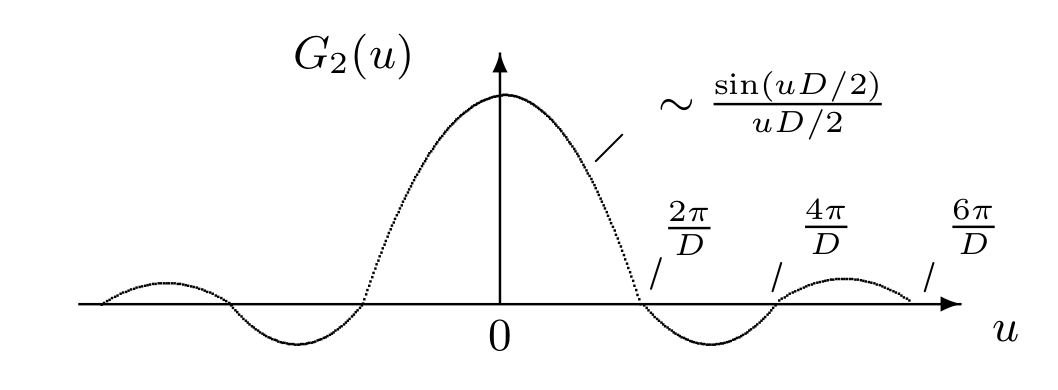
\includegraphics[width=\linewidth]{4}
	\caption{К объяснению интерференции
поляризованных лучей}
	\label{ris 4}
\end{wrapfigure}


Тонкие двоякопреломляющие пластинки, помещённые между поляроидами, кажутся окрашенными. Эта окраска может быть истолкована как результат интерференции поляризованных лучей. На рис. 4 представлена схема для
случая скрещенных поляроидов.

Здесь $ p1p'1 $ --- разрешённое направление колебаний поляризатора
(первого поляроида); $ x, y $ --- координатная система, связанная с главны-
ми направлениями двоякопреломляющей пластинки; $ p2p'2 $ --- разрешённое направление колебаний анализатора (второго поляроида). Волны
$ E_x  $ и $ E_y $ на выходе из пластинки когерентны, но не могут интерферировать, так как $ E_x \perp  E_y $. Волны $ E_1 $ и $ E_2 $ на выходе второго поляроида
также являются когерентными и к тому же поляризованы в одной плоскости. Эти волны интерферируют между собой. Результат интерференции определяется зависящим от длины волны сдвигом фаз между $ E_1 $
и $ E_2 $. В результате интерференции поляризованных лучей пластинка, освещаемая белым светом, кажется окрашенной.

Если поворачивать двоякопреломляющую пластинку, расположенную между
скрещенными поляроидами, то соотношение амплитуд волн $ E_1 $ и $ E_2 $ и разность фаз между ними не изменяются. Это означает, что цвет пластинки при её поворотах не меняется, а меняется только интенсивность света. За один оборот пластинки интенсивность четыре раза обращается в нуль --- это происходит при совпадении главных направлений
$ x $ и $ y $ с разрешёнными направлениями колебаний поляроидов.

Если же двоякопреломляющую пластинку оставить неподвижной, а
второй поляроид повернуть так, чтобы разрешённые направления $ p1p'1 $
и $ p2p'2 $ совпали, то волны $ E_1 $ и $ E_2 $ приобретают дополнительный фазовый сдвиг на $ \pi $ для всех спектральных компонент; при этом их амплитуды изменятся так, что цвет пластинки изменится на дополнительный. 
